\section{Background}
\label{sect.background}

Distributed systems are conventionally modeled as a set of \emph{nodes} (or \emph{processes}) that
can communicate only by sending and receiving messages over a network. In practice, nodes may be
servers in datacenters, end-user devices such as laptops and smartphones, or any other kind of
device with network connectivity. We assume that messages sent via the network may be delayed,
reordered, or lost entirely~-- an assumption that matches the behavior of networks in practice
\cite{Bailis:2014jx}.

Moreover, nodes or network links may fail at any time, and the non-faulty parts of the system need
to continue working in spite of such partial failures. Programming such systems is far more
difficult than writing programs that execute on a single machine. Consequently, it is valuable for
application developers to have access to abstractions that simplify the development of distributed
programs. The \emph{collaborative editing} (or \emph{data synchronization}) model discussed in this
paper is an example of such an abstraction.

The goal of an abstraction for distributed programming is to provide certain guarantees that hold in
all possible executions of a system, so that higher-level programs may rely on the abstraction
without having to worry about how it is implemented. In this paper, the abstraction we discuss is
\emph{replicated data}, that is, ensuring that each replica node has a local copy of some data
structure (such as a document). Each node may independently read and modify the data, and any
updates (modifications) are propagated to other replicas via the network.

\subsection{Consistency Models for Replicated Data}

The purpose of replication is to ensure that you have a copy of the same data on each node that is
acting as a replica. However, when multiple nodes are concurrently reading and modifying the data,
they do not have a single shared view of the data, since each node only has direct access to its
local storage, and can observe the state of another node only by exchanging messages with it via the
unreliable network \cite{Sheehy:2015jm}.

For this reason, it is likely that at any given moment in time, two replicas are not in the same
state, for example because one has received a message that has not yet been delivered to the other.
A replication algorithm must ensure that nevertheless, all replicas eventually end up in the same
state. In order to describe how and when this happens, a \emph{consistency model} defines the
guarantees provided by the replication algorithm.

\subsubsection{Strong and Eventual Consistency}

There is a spectrum of consistency models that are used in practice
\cite{Terry:1994fp}, with the two extremes of the spectrum being \emph{strong} and \emph{eventual}
consistency, respectively:

\begin{description}
\item[Strong consistency] in the context of replicated data is usually understood as linearizability
\cite{Herlihy:1990jq,Gilbert:2002il}. A linearizable system can be informally described as follows:
each operation takes effect atomically at one moment in time, and concurrent operations behave as if
there were only one copy of the data, even if in reality each replica has a separate copy. In
particular, after a write has completed, all subsequent reads must return the written value (or a
later one), since that is the behavior of a single memory location without caching or buffering. In
the context of databases, strong consistency typically refers to serializable isolation and
transaction atomicity \cite{Davidson:1985hv}.
\item[Eventual consistency] is less formally defined than linearizability, but is usually described
as ``if no new updates are made to an object, eventually all reads will return the last updated
value'' \cite{Bailis:2013jc,Burckhardt:2014hy,Terry:1994fp,Vogels:2009ca}. However, this property is
very weak: it does not define what happens if the updates to the object never cease, nor does it
constrain the values that reads may return before consistency is eventually reached.
\end{description}

The spectrum of consistency models exists due to a trade-off: systems with stronger guarantees may
have lower performance or be less fault-tolerant than systems with weaker guarantees
\cite{Davidson:1985hv,Terry:1994fp,Gilbert:2002il}. However, it is possible to strengthen the
guarantees of eventual consistency without incurring the costs inherent in strong consistency.

\subsubsection{Strong Eventual Consistency (SEC)}

One such intermediate consistency model for replicated data is \emph{strong eventual consistency} or
SEC \cite{Shapiro:2011un}. It has performance and fault-tolerance characteristics that are similar
to eventual consistency, but provides stronger guarantees. An algorithm providing SEC is defined as
satisfying the following properties:

\begin{description}
\item[Convergence:] Correct replicas that have delivered the same updates have equivalent state.
\item[Eventual delivery:] An update delivered at some replica is eventually delivered to all correct
replicas.
\item[Termination:] All executions of the algorithm eventually terminate.
\end{description}

A node is defined to be \emph{correct} if it is not faulty, i.e. if it does not crash and if it is
not permanently disconnected from the network. Although the network may be interrupted for periods
of time, a correct node will eventually be able to communicate with other correct nodes, and so the
eventual delivery property can be achieved by re-sending messages until they arrive. A faulty node
is by definition not required to deliver any messages. Termination is also straightforward to show
for many algorithms.

Thus, the key correctness property for SEC is \emph{convergence}. It is a safety property
\cite{Alpern:1985dg}~-- that is, it must hold at every point in the execution: whenever two replicas
have seen the same set of updates, but perhaps in a different order, they must be in an equivalent
state. Two states are equivalent if all reads return the same result in both states. Convergence is
much stronger than eventual consistency, a liveness property, since eventual consistency does not
constrain the values that reads may return until such time as consistency is eventually reached
\cite{Bailis:2013jc}.

\subsubsection{Asynchronous System Model}

In this paper, we discuss an approach for achieving SEC in \emph{asynchronous} systems. In the
asynchronous system model, we make no timing assumptions at all: messages may suffer unbounded
network delays, and nodes may stop executing for unbounded periods of time or fail completely
\cite{Cachin:2011wt}. Our formal definition of the asynchronous model appears in
Section~\ref{sect.network}.

Although most practical systems have fairly low network delay and fairly brief execution pauses most
of the time \cite{Bailis:2014jx}, the asynchronous model is a useful lower bound for the assumptions
that a distributed algorithm may make. Any algorithm that is proved correct under the assumptions of
the asynchronous model is also guaranteed to be correct in a system that provides stronger
guarantees, for example around timing and reliability.

Some guarantees cannot be provided in the asynchronous model; for example, there is no consensus
algorithm that is guaranteed to terminate in this system model \cite{Fischer:1985tt}. On the other
hand, consensus becomes possible if the algorithm is allowed to make certain weak timing assumptions
\cite{Chandra:1996cp}. However, SEC \emph{can} be achieved in the asynchronous model, so we use it
here in order to keep our assumptions minimal.


\subsection{Collaborative Editing and Data Synchronization}


% Upon a replica updating some subcomponent of the system's shared state, strict consistency
% guarantees that all other replicas immediately see this update. This is a strong requirement, and
% for many distributed systems is often impossible to implement due to physical constraints---notice
% of updates to the system's shared state may take significant amounts of time to percolate to
% geographically widely separated replicas, for instance. Further, in cases where one is able to
% achieve strict consistency, updates to the system's shared state may require global locks, or some
% other performance-degrading mechanism deemed unacceptable to the architects of the system. These
% problems with strict consistency motivate various relaxed consistency models, including eventual
% consistency.

% Naturally, eventual consistency requires a means of addressing conflicts when concurrent updates
% to the system's state are detected, and different strategies may be deployed, dependending on the
% requirements of the particular system. Popular strategies include invoking a user-specified
% conflict resolution handler upon detection of conflicts, or uniformly applying a \emph{last writer
% wins} policy to all conflicts. These strategies are often \emph{ad hoc} and error prone,
% motivating strong eventual consistency.

% We prove this convergence property in an abstract setting, that is, any two arbitrary list of
% distinct events, enriched by an order relation that satisfies a \emph{consistency property},
% converge.

\begin{figure}
\centering
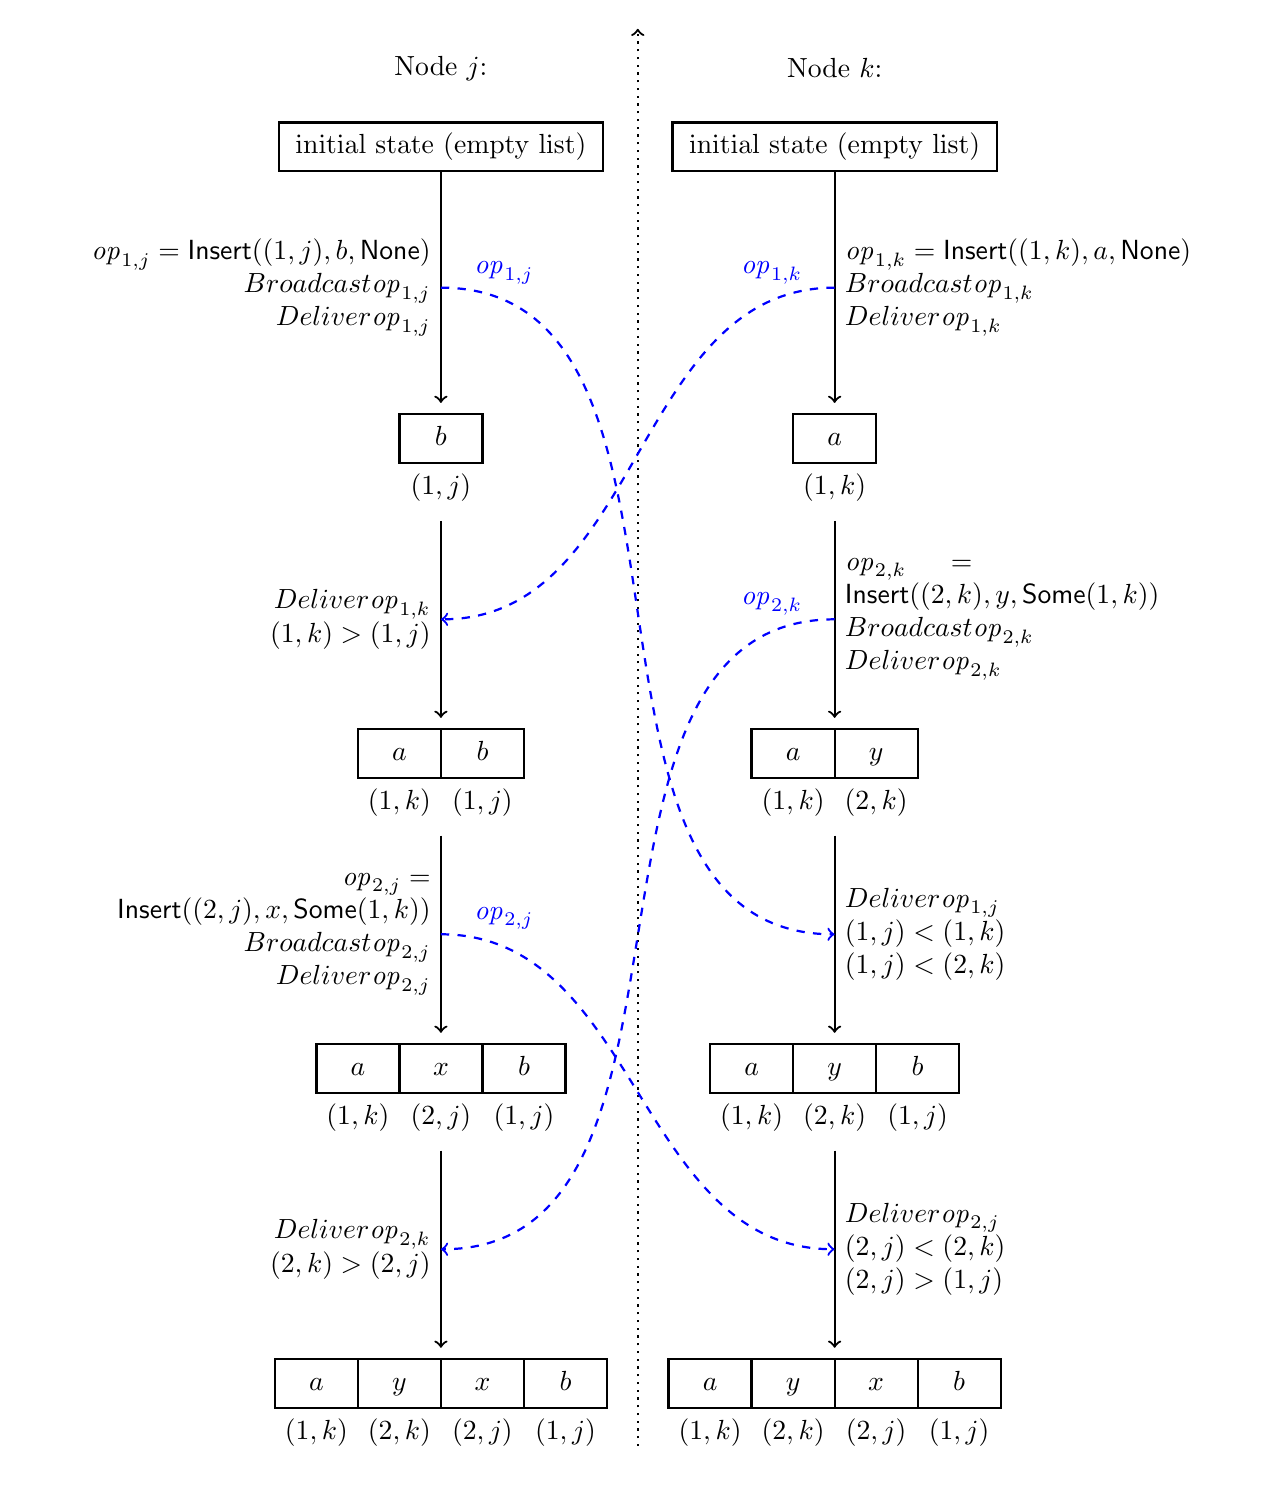
\begin{tikzpicture}[auto,scale=1.0]
\onehalfspacing
\path [draw,dotted] (2.5,-0.5) -- (2.5,17.5);

\tikzstyle{initstate}=[rectangle,draw,inner xsep=6pt,text height=8pt,text depth=3pt]
\tikzstyle{state}=[matrix,column sep={30pt,between origins}]
\tikzstyle{val}=[draw,anchor=base,minimum width=30pt,text height=8pt,text depth=3pt]
\tikzstyle{oid}=[anchor=base]
\tikzstyle{leftevent}=[left,text width=5cm,text ragged left,midway]
\tikzstyle{rightevent}=[right,text width=5cm,text ragged,midway]
\tikzstyle{every path}=[thick,->]

\node (leftR) at (0,17) {Node $j$:};
\node (left1) at (0,16) [initstate] {initial state (empty list)};
\node (left2) at (0,12) [state] {
    \node [val] {$b$};     \\
    \node [oid] {$(1,j)$}; \\
};
\node (left3) at (0,8) [state] {
    \node [val] {$a$};     & \node [val] {$b$};     \\
    \node [oid] {$(1,k)$}; & \node [oid] {$(1,j)$}; \\
};
\node (left4) at (0,4) [state] {
    \node [val] {$a$};     & \node [val] {$x$};     & \node [val] {$b$};     \\
    \node [oid] {$(1,k)$}; & \node [oid] {$(2,j)$}; & \node [oid] {$(1,j)$}; \\
};
\node (left5) at (0,0) [state] {
    \node [val] {$a$};     & \node [val] {$y$};     & \node [val] {$x$};     & \node [val] {$b$};     \\
    \node [oid] {$(1,k)$}; & \node [oid] {$(2,k)$}; & \node [oid] {$(2,j)$}; & \node [oid] {$(1,j)$}; \\
};

\draw (left1) -- (left2) node (send1j) [leftevent] {
    \hfill $\mathit{op}_{1,j} = \mathsf{Insert}((1, j), b, \mathsf{None})$ \\
    \hfill $\text{Broadcast } \mathit{op}_{1,j}$ \\
    \hfill $\text{Deliver } \mathit{op}_{1,j}$ \\
};
\draw (left2) -- (left3) node (recv1k) [leftevent] {
    \hfill $\text{Deliver } \mathit{op}_{1,k}$ \\
    \hfill $(1,k) > (1,j)$ \\
};
\draw (left3) -- (left4) node (send2j) [leftevent] {
    \hfill $\mathit{op}_{2,j} = \mathsf{Insert}((2, j), x, \mathsf{Some}(1,k))$ \\
    \hfill $\text{Broadcast } \mathit{op}_{2,j}$ \\
    \hfill $\text{Deliver } \mathit{op}_{2,j}$ \\
};
\draw (left4) -- (left5) node (recv2k) [leftevent] {
    \hfill $\text{Deliver } \mathit{op}_{2,k}$ \\
    \hfill $(2,k) > (2,j)$ \\
};

\node (rightR) at (5,17) {Node $k$:};
\node (right1) at (5,16) [initstate] {initial state (empty list)};
\node (right2) at (5,12) [state] {
    \node [val] {$a$};     \\
    \node [oid] {$(1,k)$}; \\
};
\node (right3) at (5,8) [state] {
    \node [val] {$a$};     & \node [val] {$y$};     \\
    \node [oid] {$(1,k)$}; & \node [oid] {$(2,k)$}; \\
};
\node (right4) at (5,4) [state] {
    \node [val] {$a$};     & \node [val] {$y$};     & \node [val] {$b$};     \\
    \node [oid] {$(1,k)$}; & \node [oid] {$(2,k)$}; & \node [oid] {$(1,j)$}; \\
};
\node (right5) at (5,0) [state] {
    \node [val] {$a$};     & \node [val] {$y$};     & \node [val] {$x$};     & \node [val] {$b$};     \\
    \node [oid] {$(1,k)$}; & \node [oid] {$(2,k)$}; & \node [oid] {$(2,j)$}; & \node [oid] {$(1,j)$}; \\
};

\draw (right1) -- (right2) node (send1k) [rightevent] {
    $\mathit{op}_{1,k} = \mathsf{Insert}((1, k), a, \mathsf{None})$ \\
    $\text{Broadcast } \mathit{op}_{1,k}$ \\
    $\text{Deliver } \mathit{op}_{1,k}$ \\
};
\draw (right2) -- (right3) node (send2k) [rightevent] {
    $\mathit{op}_{2,k} = \mathsf{Insert}((2, k), y, \mathsf{Some}(1, k))$ \\
    $\text{Broadcast } \mathit{op}_{2,k}$ \\
    $\text{Deliver } \mathit{op}_{2,k}$ \\
};
\draw (right3) -- (right4) node (recv1j) [rightevent] {
    $\text{Deliver } \mathit{op}_{1,j}$ \\
    $(1,j) < (1,k)$ \\
    $(1,j) < (2,k)$ \\
};
\draw (right4) -- (right5) node (recv2j) [rightevent] {
    $\text{Deliver } \mathit{op}_{2,j}$ \\
    $(2,j) < (2,k)$ \\
    $(2,j) > (1,j)$ \\
};

\begin{scope}[dashed,blue]
    \tikzstyle{every node}=[text centered]
    \draw (send1j.east) to [out=0,in=180] (recv1j.west);
    \draw (send2j.east) to [out=0,in=180] (recv2j.west);
    \draw (send1k.west) to [out=180,in=0] (recv1k.east);
    \draw (send2k.west) to [out=180,in=0] (recv2k.east);
    \node at (0.8,14.4) {$\mathit{op}_{1,j}$};
    \node at (0.8, 6.2) {$\mathit{op}_{2,j}$};
    \node at (4.2,14.4) {$\mathit{op}_{1,k}$};
    \node at (4.2,10.2) {$\mathit{op}_{2,k}$};
\end{scope}
\end{tikzpicture}

\caption{RGA example}\label{fig.two-lists}
\end{figure}
